%********************************************************************
% Appendix
%*******************************************************
% If problems with the headers: get headings in appendix etc. right
%\markboth{\spacedlowsmallcaps{Appendix}}{\spacedlowsmallcaps{Appendix}}
\chapter{Appendix E: Supplementary Information of Chapter 7}

\begin{refsection}[referencesCh7]

\section{Literature review}
The literature available referred to CO\textsubscript{2} capture is extensive, not only for combustion processes also for the particular case of biogas upgrading, there exists a lack of literature regarding the selection of the most appropriate biogas upgrading technology. It should be noted that the goal of this work it is not limited to the optimization the biogas production and upgrading processes, which it is implicitly done in the work, but the aim pursued is to determine the optimal biogas upgrading technology among the different feasible processes.

This lack in the literature was detected after a literature review, carried out with special emphasis in specific studies about biogas upgrading. On one hand, as a result of the literature review made, it could be concluded that the literature about reviews of biogas upgrading processes is extensive, even when only recent works are considered, as it is shown in Table \ref{table:ChETable1}. On the other hand, just a few recent works are approaching to carry out a systematic comparison of the processes, such as the work of \citet{collet2017techno}, where a comparison of several CO\textsubscript{2} capture technologies using experimental data from other studies is presented, but without  integrating and optimizing the biogas production and upgrading processes, or the study of \citet{vo2018techno}, where simulations of biogas upgrading processes limited to amine scrubbing and biological methanation are carried out, not including some essential upgrading technologies such as membranes or PSA. Other works, including but not limited to \citet{capra2018biogas, curto2019renewable, gilassi2019optimizing}, determine the optimal biogas upgrading process but analyzing only one technology in each case (amines scrubbing, biogas methanation, and membrane separation). In the work presented, 5 technologies have been evaluated considering both heuristic and mathematical modelling stages (biogas methanation, water scrubbing, pressure swing adsorption systems, amines scrubbing, and membranes separation systems).

\begin{table}[h]
	\centering
	\caption{Relevant literature for biogas upgrading.}
	\label{table:ChETable1}
	\resizebox{\columnwidth}{!}{
		\begin{tabular}{@{}cc@{}}
			\toprule
			Author                        & Study performed                                                              \\ \midrule
			\protect\citet{angelidaki2018biogas}       & Review of biogas upgrading technologies                                      \\
			\protect\citet{awe2017review}              & Review of biogas upgrading technologies                                      \\
			\protect\citet{bauer2013biogas}          & Review of biogas upgrading technologies                                      \\
			\protect\citet{khan2017biogas}             & Review of biogas upgrading technologies                                      \\
			\protect\citet{miltner2017review}          & Review of biogas upgrading technologies                                      \\
			\protect\citet{sun2015selection}              & Review of biogas upgrading technologies                                      \\
			\protect\citet{zhou2017alternative}             & Review of biogas upgrading technologies                                      \\
			\protect\citet{collet2017techno}           & Techno-economic and life cycle assessment of biogas upgrading                \\
			\protect\citet{ferella2019techno}          & Techno-economic assesment of strategic plans for biogas upgrading plants     \\
			\protect\citet{toledo2017comparative} & Comparison of photosynthetic and physico-chemical biogas upgrading processes \\
			\protect\citet{vo2018techno}               & Simulation of amine scrubbing and biological methanation                     \\
			\protect\citet{capra2018biogas}            & Optimal selection of amine scrubbing process for biogas upgrading            \\
			\protect\citet{curto2019renewable}        & Optimal selection of renewable biogas methanation processes                  \\
			\protect\citet{filipetto2019optimization}        & Optimal selection of membrane separation process for biogas upgrading        \\
			\protect\citet{gilassi2019optimizing}          & Optimal selection of membrane separation process for biogas upgrading        \\
			\protect\citet{morero2017evaluation}           & Optimal selection of amine scrubbing process for biogas upgrading            \\ \bottomrule
		\end{tabular}
	}
\end{table}

\begin{figure}[h]
	\centering
	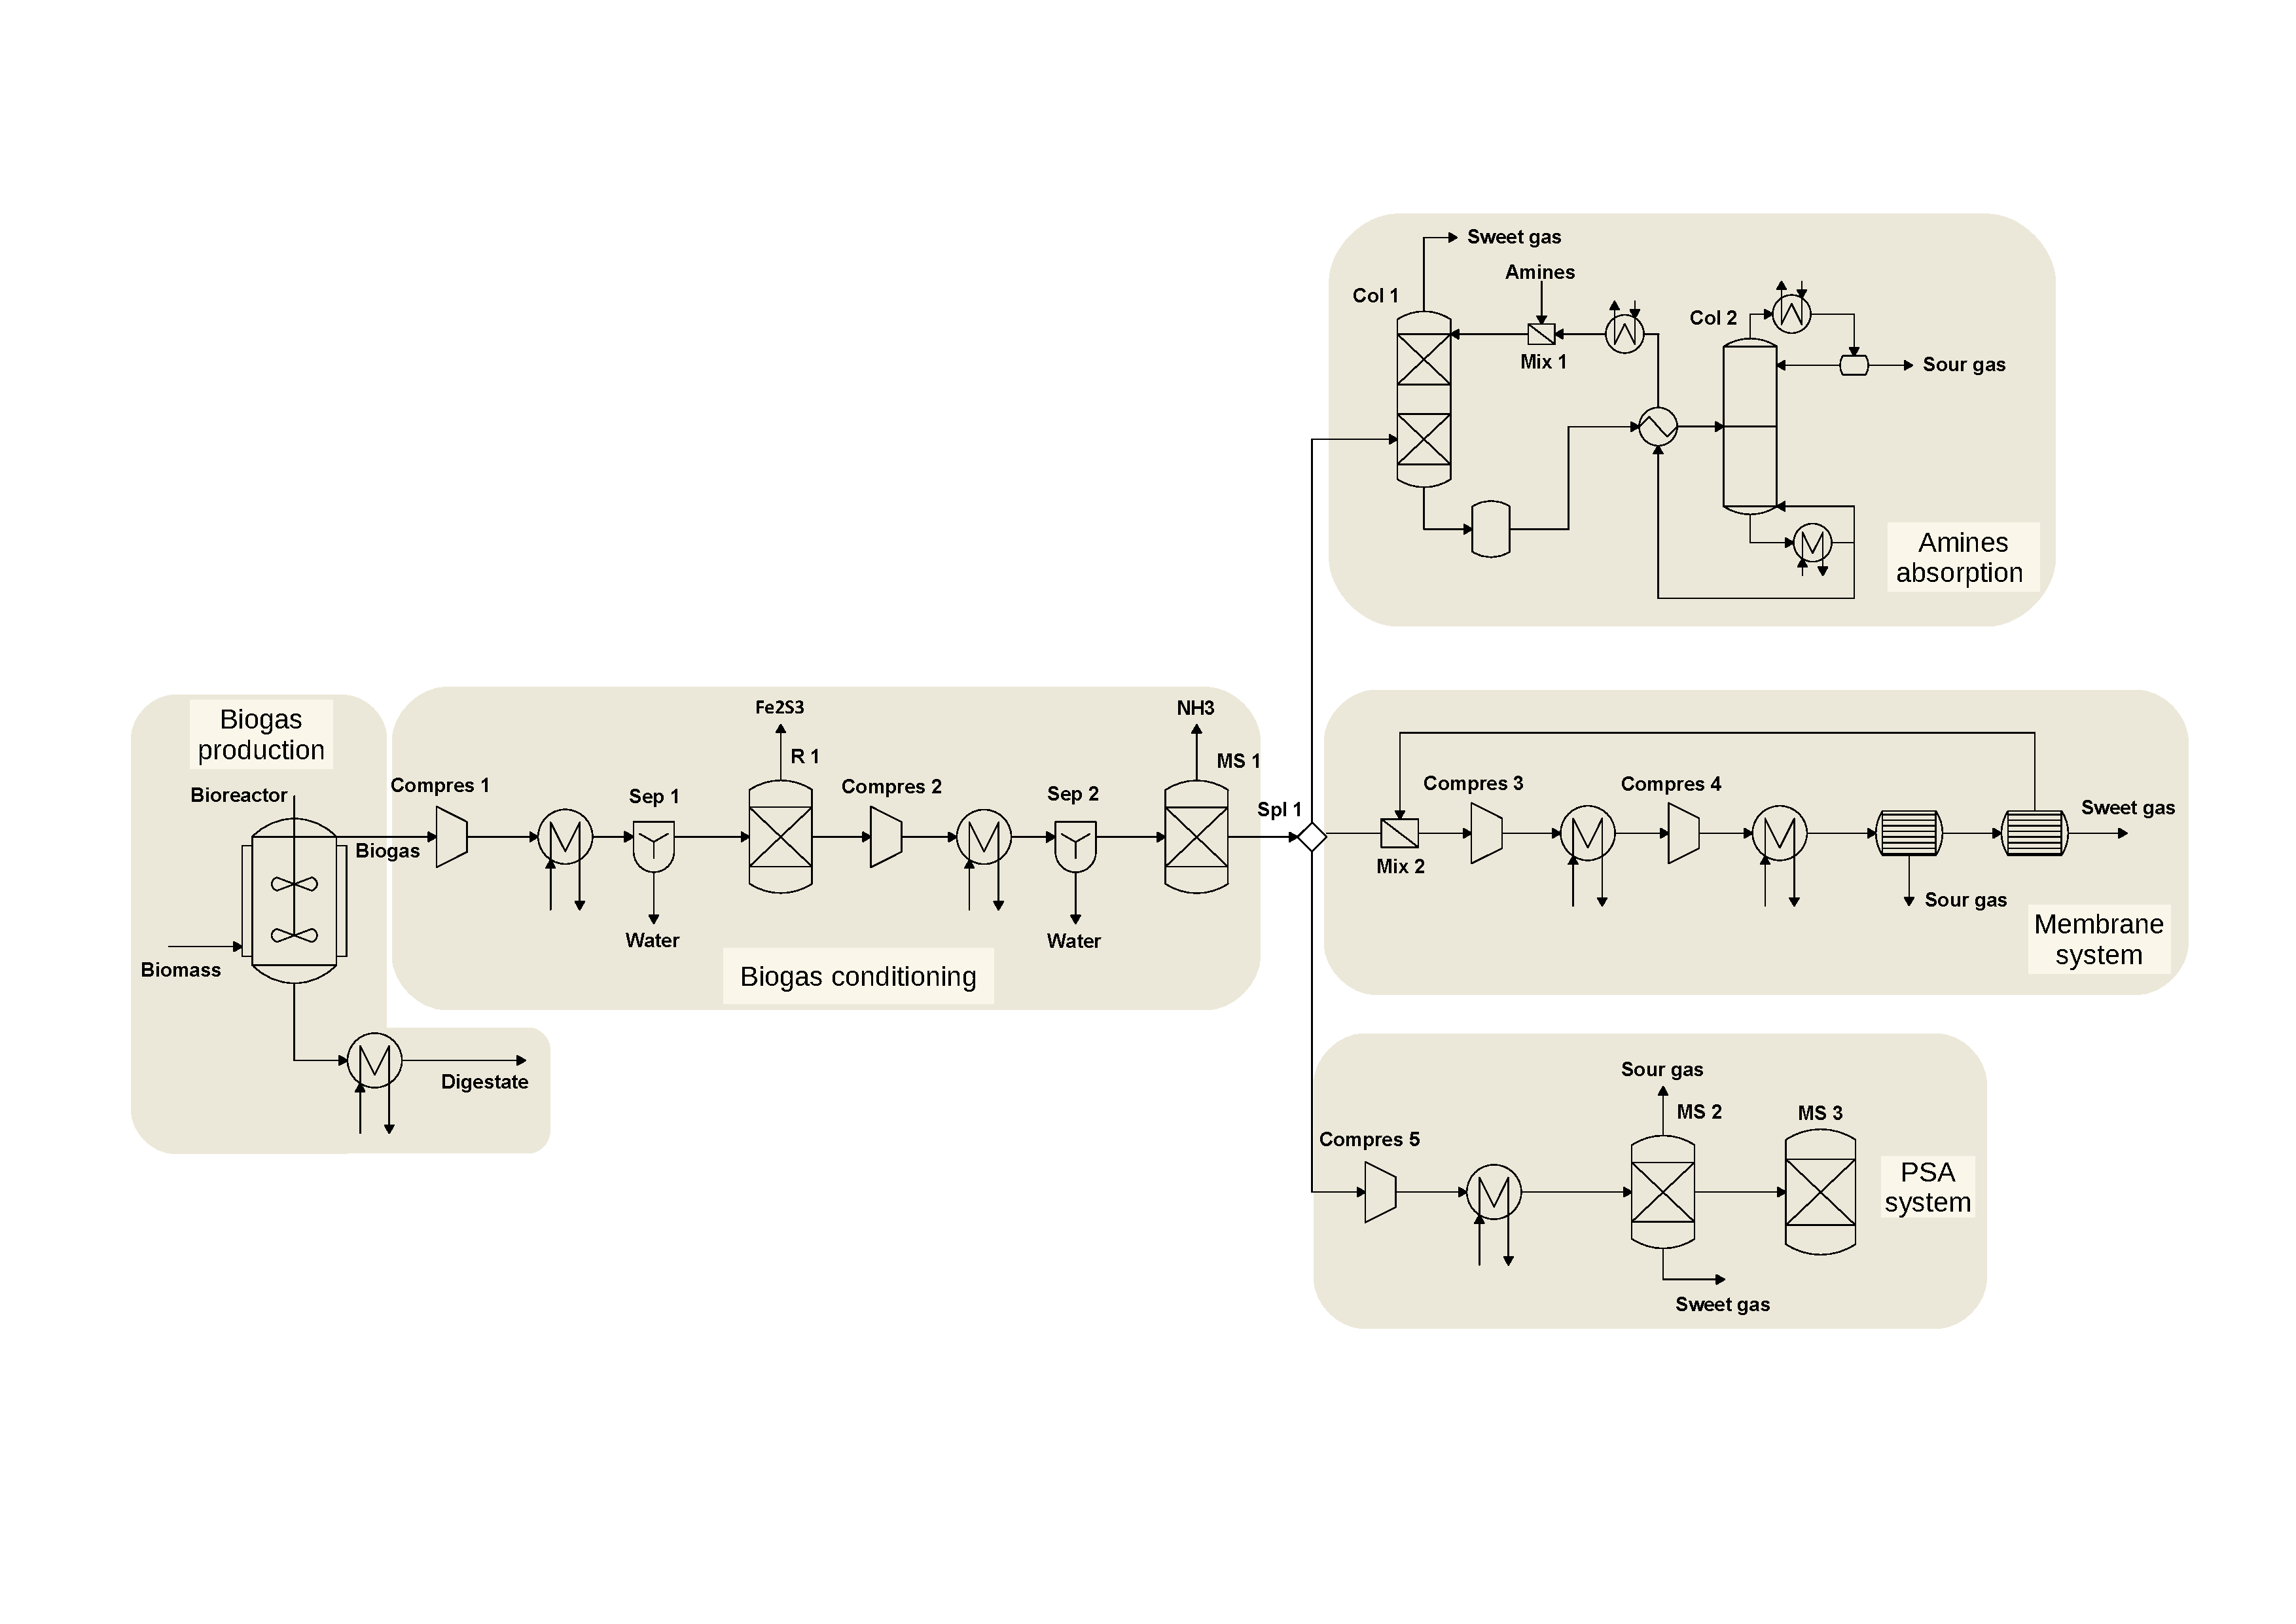
\includegraphics[width=1\linewidth, trim={3cm 7cm 3cm 5cm},clip]{gfx/Chapter7/Figure2.pdf} 
	\caption{Scheme of the proposed superstructure for biogas upgrading into biomethane.}
	\label{fig:ChEFig1}
\end{figure}

\section{Modelling approach} \label{section:SuppMatPaperCO2Section2}
\subsection{Amines} \label{section:SuppMatAmines}
The CO\textsubscript{2} absorption systems using amines typically operate at low temperatures, around 25-30 \textdegree C, and partial pressures above 0.05 bar, reaching removal yields of 90\%-95\% \citep{zhang2013modeling}. In contrast to postcombustion gases, which contains large amounts of nitrogen from air, biogas is composed mainly by methane and CO\textsubscript{2}, resulting in higher carbon dioxide partial pressures and in the need for lower operating pressures. CO\textsubscript{2} partial pressures above 0.1 bar have been assumed to secure high removal yields \citep{zhang2013modeling}, resulting in the need to operate at total pressures around 1-1.5 bar to secure the appropriate CO\textsubscript{2} partial pressures \citep{movagharnejad2011simulation, xue2017comparative}. 

The total amount of solution of amines needed to absorb the CO\textsubscript{2} from the gas stream is calculated as a function of the amount of sour gases eliminated, Eq. \ref{eq:ChEEq1}. According to \citet{2012gpsa}, the concentration of solution and the correction factor ($GPSA$) depend on the amine used, as is shown in Table \ref{table:ChETable2}. The flow of the amine solutions depends on their solubility. Thus, for a fixed removal ratio, the amines solution flow required changes from one to another. It is considered there is no methane absorption in the amines flow, therefore all biomethane entering in the unit leaves the column and it is sent to storage.

\begin{align}
fc_{amine} = \frac{{MW}_{amine}}{\left[ {amine} \right]}\cdot\left( \frac{CO_{2_{eff}} \cdot fc_{CO_2}}{MW_{CO_2}} \right)\cdot\left( {\frac{1}{{{{GPSA}}}}} \right)  \label{eq:ChEEq1}
\end{align}

The solution of amine used in column 1 comes from two sources, as it shown in Eq. \ref{eq:ChEEq2}, i.e., the amines from the regeneration column (column 2 in Figure 1), and some make-up solution to replace the amine losses with the gas outlet stream in the regeneration column. Additionally, to mix the two streams of amines at the same temperature, a heat exchanger is used to adjust the temperature of the amine flow stream which leaves the regeneration column to 25 \textdegree C.

\begin{align}
fc_{amine} =  fc_{recycled \ amine}  + fc_{fresh \ amine} \label{eq:ChEEq2}
\end{align}

The mixing of the two amines streams is assumed to be adiabatic. The energy balance to the heat exchanger is as follows, Eq. \ref{eq:ChEEq3}.

\begin{align}
Q = F_{amine} \cdot q_{heat,amine} \label{eq:ChEEq3}
\end{align}

Where $F_{amine}$ is referred to the total mass flow of the amines stream, and qamine the heat flow ratio based on the rules of thumb reported by \citet{2012gpsa}. The values are collected in Table \ref{table:ChETable2}.	

The assumed CO\textsubscript{2} removal efficiency in the absorption column is 0.95, based on literature data \citep{zhang2013modeling}. The sour gas is absorbed by the amines in the absorption column, being withdrawn from the gas phase. The absorption is an exothermic process. Therefore, this energy is to be refrigerated, and the operation of the column is isothermal, Eq. \ref{eq:ChEEq4}. The heats of reaction are shown in Table \ref{table:ChETable3}.

\begin{align}
Q_{Col1} = \Delta H_{react, amine} \cdot CO_{2_{eff}} \cdot fc_{CO_2} \label{eq:ChEEq4}
\end{align}

The biomethane leaves the column and it is sent to storage. On the other hand, the amine with the CO\textsubscript{2} absorbed is sent to the regeneration column (column 2). The solution is heated up before being fed to column 2 through the heat transfer from the amines stream leaving the reboiler of the regeneration column with the aim of improving the desorption process. Rules of thumb reported in the literature are used to compute the energy involved in the heat exchanger using Eq. \ref{eq:ChEEq6}, considering the corresponding values of qamine collected in Table \ref{table:ChETable3}. 

The operation of column 2 is also based on rules of thumb \citep{2012gpsa, 2004gpsa} including the estimation of the energy consumption in the reboiler and the cooler refrigeration requirements. According to the literature, the inlet temperature to column 2, $T_{Col2}$, is equal to 93 \textdegree C, whereas the temperature of the outlet amines stream, $T_{bottom}$, is equal to 125 \textdegree C, while at the condenser, the temperature, $T_{top}$, is equal to 54 \textdegree C. Thus, the energy balances of the stream entering column 2 are described in Eq. \ref{eq:ChEEq5}.

\begin{align}
\begin{array}{l} Q_{Cond} = F_{Cond} \cdot q_{Cond,amine} \\ Q_{Reb} = F_{Reb} \cdot q_{Reb,amine}\end{array} \label{eq:ChEEq5}
\end{align}

From the reboiler, the regenerated amine is cooled down heating up the feed to the column, Eq. \ref{eq:ChEEq6}.

\begin{align}
Q_{Cooling} = F_{Cooling} \cdot q_{Cooling,amine} \label{eq:ChEEq6}
\end{align}

The gas leaving the regeneration column is saturated with the amines aqueous solution, producing the losses of amines which have to be replaced before be recirculated to the absorption column. In order to calculate these losses, humidification models are used. First, the saturation pressure of the amine solution is calculated, Eq. \ref{eq:ChEEq7}. Then, the specific humidity of the gaseous stream is computed to determine the amount of amines solution accompanying the CO\textsubscript{2} gaseous stream which leaves the regeneration column, Eq. \ref{eq:ChEEq8}, where the operating pressure of the regeneration column, $P_{Col2}$, is equal to 1.7 bar \citep{2004gpsa}. As an approximation, it is assumed that the amine solution behaves as water. The amount of amine lost with the sour gases is the one to be fed as fresh amine.

\begin{align}
P_{amines \ solution} = Exp \left( A - \frac{B}{\left( C + {T}_{top} \right)} \right) \label{eq:ChEEq7}
\end{align}

\begin{align}
Y = \frac{MW_{Wa}}{MW_{outlet \ gas}} \cdot \frac{P_{amines \ solution}}{\left( P_{Col2} - P_{amines \ solution} \right)} \label{eq:ChEEq8}
\end{align}

Three different amines are selected aiming a high selectivity, MEA, DEA, and MDEA. Table \ref{table:ChETable2} shows the parameters used in the amines absorption modelling for each amine considered \citep{2012gpsa, 2004gpsa}.

\begin{table}[h]
	\centering
	\caption{Amine properties for CO\textsubscript{2} capture \protect\citet{2012gpsa, 2004gpsa}.}
	\label{table:ChETable2}
%	\resizebox{\columnwidth}{!}{
		\begin{tabular}{@{}cccc@{}}
			\toprule
			& MEA     & DEA       & MDEA     \\ \midrule
			Gas pickup (mol/mol\textsubscript{amine})       & 0.35    & 0.35-0.65 & 0.2-0.55 \\
			Solution concentration (wt \%) & 20      & 35        & 45       \\
			Heat of reaction (BTU/lb CO\textsubscript{2})  & 620-700 & 580-650   & 570-600  \\
			GPSA                           & 0.35    & 0.50      & 0.38     \\
			Density                        & 1.01    & 1.05      & 1.05     \\
			Cost (EUR/kg)                  & 1.30    & 1.32      & 3.09     \\
			Molecular weight               & 61      & 105       & 119      \\ \bottomrule
		\end{tabular}
%		\begin{tablenotes}
%			\item[a] \\Insert footnote here
%		\end{tablenotes}
%	}
\end{table}

\begin{table}[h]
	\centering
	\caption{Amine regeneration heat loads \protect\citet{2004gpsa}.}
	\label{table:ChETable3}
	%	\resizebox{\columnwidth}{!}{
	\begin{tabular}{@{}cc@{}}
		\toprule
		& Duty (BTU/hr) \\ \midrule
		Reboiler                   & 72000 GPM     \\
		Condenser                  & 30000 GPM     \\
		Amine feed to distillation & 45000 GPM     \\
		Amine cooler               & 15000 GPM     \\ \bottomrule
	\end{tabular}
	%	}
\end{table}

The biomethane production model through amines scrubbing includes the units described in sections \ref{section:BiogasProductionPaperBiogas} and \ref{section:SuppMatAmines}. The NLP problem consists of 288 equations and 953 variables per amine evaluated and is solved using a multistart initialization approach with CONOPT as the preferred solver where the main decision variable are the pressures temperatures and flow rates.

\subsection{PSA} \label{section:SuppMatPSA}
The stream of gases passes through the bed of zeolites and the carbon dioxide is captured by adsorption. The system consists of the compression train and the zeolite beds. 

The adsorption capacity of the zeolites is directly related to the partial pressure of the CO\textsubscript{2}. Therefore, a system of compressors with intermediate cooling is implemented to determine the optimal operating pressure. As it is described previously, the compressors are modelled assuming polytropic behavior, with a polytropic coefficient $z$ of 1.4 and an efficiency of the compression stages of 0.85, Eq. \ref{eq:ChEEq9}. 

\begin{align}
\begin{array}{l}{T_{out/compresor}} = {T_{in/compressor}} + {T_{in/compressor}}\left( {{{\left( {\frac{{{P_{out/compressor}}}}{{{P_{in/compressor}}}}} \right)}^{\frac{{z - 1}}{z}}} - 1} \right)\frac{1}{{{\eta _c}}}\\{{{W}}_{\left( {Compressor} \right)}} = \left( F \right)\cdot\frac{{R\cdot z\cdot\left( {{{{T}}_{in/compressor}}} \right)}}{{\left( {\left( {{{M}}w} \right)\cdot\left( {z - {{1}}} \right)} \right)}}\frac{1}{{{\eta _c}}}\left( {{{\left( {\frac{{{P_{out/compressor}}}}{{{P_{in/compressor}}}}} \right)}^{\frac{{z - 1}}{z}}} - {{1}}} \right)\end{array} \label{eq:ChEEq9}
\end{align}

The removal ratio is given by the breakthrough curve of the adsorbent bed. Based on experimental data \citep{hauchhum2014carbon} for adsorption stages below 20 min, the CO\textsubscript{2} removal yield of the PSA system is assumed to be 98\%, containing below 2\% CO\textsubscript{2} at the outlet stream, \citep{ferella2017separation}. The mass balance at the bed is as shown in Eq. \ref{eq:ChEEq10}.

\begin{align}
\begin{array}{l} CO_{2}{\text{ stream:}}\\{\left. {fc_{CO_{2}}} \right|_{out}} = \eta {\left. {fc_{CO_{2}}} \right|_{in}}\\{\left. {fc_{CH_{4}}} \right|_{out}} = 0.02\cdot{\left. {fc_{CH_{4}}} \right|_{in}}\\CH_{4}{\text{ stream:}}\\{\left. {fc_{CO_{2}}} \right|_{out}} = (1 - \eta ){\left. {fc_{CO_{2}}} \right|_{in}}\\{\left. {fc_{CH_{4}}} \right|_{out}} = 0.98\cdot{\left. {fc_{CH_{4}}} \right|_{in}}
\end{array} \label{eq:ChEEq10}
\end{align}

To compute the mass of bed the adsorption capacity of the bed is evaluated. Based on experimental data, the Langmuir isotherm is the adsorption model considered for this process, Eq. \ref{eq:ChEEq11}, since this is the one that best fits the performance of the zeolite 13X - CO\textsubscript{2} system \citep{hauchhum2014carbon}. 

\begin{align}
q = \frac{{{q_m}\cdot K\cdot{P_{CO_{2}}}}}{{1 + K\cdot{P_{CO_{2}}}}} \label{eq:ChEEq11}
\end{align}

Where the parameters $q_{m}$ and $K$ depend on the adsorbent material. Considering zeolite 13X, the effect of the operating temperature, within the range of 25 \textdegree C-60 \textdegree C, for both parameters can be correlated using data available in the literature, Eq. \ref{eq:ChEEq12a} \citep{hauchhum2014carbon}.

\begin{subequations}
	\begin{align} 
	%	\tag{12a}
	& 
	\begin{array}{l}q_m= -3.15551 \cdot 10^{-2}  T(\text{\textdegree C})  + 5.02915 \\ K= \left( 1.63070 \cdot 10^{-03} T(\text{\textdegree C})\right)^2- 3.68662 \cdot 10^{-1} T(\text{\textdegree C}) + 27.3737\end{array}  \label{eq:ChEEq12a}
	\\
	& \begin{array}{l} q_m=-1.82355·10^{-2}  T(\text{\textdegree C})  + 3.72021 \\ K=\ 1.63070·10^{-03}  T(\text{\textdegree C})^2- 3.68662·10^{-1}  T(\text{\textdegree C}) + 27.3737 \end{array} \label{eq:ChEEq12b}
	\end{align}
\end{subequations}

As result of the breakthrough curve for the zeolite 13X – carbon dioxide system, the operating time must be below 20 min so that the exit gas (methane) contains only traces of CO\textsubscript{2}. Similarly, correlations are developed for zeolite 4A, Eq. \ref{eq:ChEEq12b}. The operating time of zeolite 4A must be below 20 min \citep{hauchhum2014carbon}. Note that the expression for the computing of the constant K in the Langmuir correlation is the same for both adsorbents evaluated.

However, the adsorption capacity decays cycle after cycle until it stabilizes around 65\% of the initial capacity computed by Eq. \ref{eq:ChEEq13} \citep{hauchhum2014carbon}. Therefore, a corrected value for $q$ is applied to compute the amount of zeolite used in the PSA system, as it can be shown in Eq. 14, where the CO\textsubscript{2} removal yield of the PSA syste, is assumed to be 98\%, containing below 2\% CO\textsubscript{2} at the outlet stream \citep{ferella2017separation}, and $\tau$ is equal to 20 min, based on the results of \citep{hauchhum2014carbon}. Furthermore, a lifetime of the zeolites bed of 5 years has been considered based on data reported by \citet{Xiao2013}. Thus for the cost, we considered that over the 20 years life time of the plant, 5 beds will be used.

\begin{align}
\begin{array}{l}{m_{Zeolite}} = \frac{1}{{q\cdot0.65}}\frac{{f{c_{C{O_2}}}\cdot1000}}{{M{W_{(C{O_2})}}}}\eta \cdot\tau \\\end{array} \label{eq:ChEEq13}
\end{align}

In the case of the PSA system, the objective function is shown in Eq. \ref{eq:ChEEq14}. To estimate the cost of the PSA system, Eq. \ref{eq:ChEEq15}, it is assumed that the zeolite bed loses efficiency over time, resulting in a lifetime of 5 years before it needs to be replaced \citep{Xiao2013}. As the plant life is considered 20 years, the zeolites bed must be replaced 4 times during the plant life, $N_{Cycle}$. 

\begin{align}
Profit = BioCH_{4} - Cost_{Zeolite \ system} \label{eq:ChEEq14}
\end{align}

\begin{align}
Cost_{Zeolite \ system} = C_{Electricity} \cdot W_{Compressor} + \frac{1}{K}{M_{Zeolite}} \cdot {C_{Zeolite}}\cdot{N_{Cycle}} \label{eq:ChEEq15}
\end{align}

The cost of the zeolites considered is 5 USD/kg for both zeolite 13 X and zeolite 4A \citep{Xiao2013}. 
 
The production of biomethane through pressure swing adsorption includes the units described in sections \ref{section:BiogasProductionPaperBiogas} and \ref{section:SuppMatPSA} consisting of an NLP problem of 283 equations and 828 variables that is solved similarly as in the case of the selection of amines where the main decision variables are the operating pressure of the adsorption tower and the size of the bed.

\subsection{Membranes} \label{section:SuppMatMembranes}
The membrane system considered is dual-stage membrane systems with single compression stage before the membrane system and no recompression stage between membrane units, have been deemed as the most economic under a wide range of feed compositions \citep{kim2017optimization}. The compressor is modelled as presented above, assuming polytropic compression of the gas, Eq. \ref{eq:ChEEq9}. Each membrane module is modelled using mass balances, considering the permeate and retentate streams, Eqs. \ref{eq:ChEEq16} and \ref{eq:ChEEq17}, and the flux of the gases through the membrane, that is a function of the concentration gradient between both sides of the membrane, Eq. \ref{eq:ChEEq19} \citep{FernandesRodriguesMsc}. The flux is the parameter which allows computing the area of the membrane, as it is shown in Eq. \ref{eq:ChEEq18}, based on the permeability of the membrane, Eq. \ref{eq:ChEEq21}. As the driving force in the membrane separation process is the concentration gradient, the removal of CO\textsubscript{2} results in a change in the composition of the stream along the membrane, leading to a change in the driving force which controls the process. Therefore, an average molar fraction between the feed and the retentate composition is used to compute the separation driving force, Eq. \ref{eq:ChEEq20}. 

\begin{align}
F_{feed} = {F_{permeate}} + {F_{retentate}}  \label{eq:ChEEq16}
\end{align}

\begin{align}
F{}_{feed}\cdot{y_{i,feed}} = {F_{permeate}}\cdot{y_{i,permeate}} + {F_{retentate}}\cdot{y_{i,retentate}}; \ i \in (C{O_2},CH_{4}) \label{eq:ChEEq17}
\end{align}

\begin{align}
{J_i} = \frac{{{F_{permeate}}\cdot{y_{i,permeate}}}}{{{A_{membrane}}}};\ i \in (CO_{2},CH_{4}) \label{eq:ChEEq18}
\end{align}

\begin{align}
{J_i} = {\varepsilon _i}\left[ {\mathop {{y_{feedside}}}\limits^{} \cdot{P_{feed}} - {y_{i,permeate}}\cdot P{}_{Permeate}} \right]; \ i \in (CO_{2},CH_{4} \label{eq:ChEEq19}
\end{align}

\begin{align}
\mathop {{y_{feedside}}}\limits^{}  = \frac{{{y_{i,feed}} - {y_{i,retentate}}}}{{\ln \left( {\frac{{{y_{i,feed}}}}{{{y_{i,retentate}}}}} \right)}}; \ i \in (CO_{2},CH_{4}) \label{eq:ChEEq20}
\end{align}

\begin{align}
{\varepsilon _i} = \frac{{Perm_{i}}}{\delta }; \ i \in (CO_{2},CH_{4}) \label{eq:ChEEq21}
\end{align}

Where $\delta$is the membrane thickness, and ${Perm_{i}}$ the permeability of the component $i$. The usual membrane thickness for industrial units is equal to 30 nm. Three different membrane materials are selected aiming a large CO\textsubscript{2} permeability, low methane permeability, and therefore, high selectivity; cellulose acetate, polyamide, and polycarbonate. Table \ref{table:ChETable4} shows the permeabilities for each membrane material considered in the model at 25 \textdegree C \citep{vrbova2017upgrading}. The solution of the optimization problem will yield intermediate conditions to assure natural gas composition of the biomethane.

\begin{table}[h]
	\centering
	\caption{Gases permeability \protect\citet{vrbova2017upgrading}.}
	\label{table:ChETable4}
	%	\resizebox{\columnwidth}{!}{
	\begin{tabular}{@{}ccc@{}}
		\toprule
		& \multicolumn{2}{c}{Permeability (Barrer)} \\ \midrule
		Polymer           & CH4                 & CO2                 \\
		Cellulose acetate & 0.21                & 6.30                \\
		Polycarbonate     & 0.13                & 4.23                \\
		Polyimide         & 0.25                & 10.7                \\ \bottomrule
	\end{tabular}
	%	}
\end{table}

Finally, the simplified profit objective function for the membrane separation system, Eq. \ref{eq:ChEEq22}, considers cost of the gas compression and the amortization of the investment costs of the membranes, Eq. \ref{eq:ChEEq23}. 

\begin{align}
Profit = BioCH_{4} - Cost_{{{Membrane \ system}}} \label{eq:ChEEq22}
\end{align}

Eq21
\begin{align}
& Cost_{{{Membrane \ system}}} = \nonumber \\
& {{{C}}_{Electricity}}\cdot W_{Compressor} + \frac{1}{K}\cdot{C_{Membrane}}\cdot\frac{1}{{Lf}}\cdot{N_{Membranes}}(\sum\limits_{i \in stages} {Are{a_i}} ) \label{eq:ChEEq23}
\end{align}

A value of 50 USD/m\textsuperscript{2} will be used based on the literature \citep{kim2017optimization}. Considering the plant life equal to 20 years, the membranes with a typical lifetime of 4 years must be replaced 5 times during the plant life, $N_{Membranes}$ \citep{scholz2015structural}.

The biogas production and upgrading considering a membranes separation system is formulated as an NLP problem considering the units described in sections \ref{section:BiogasProductionPaperBiogas} and \ref{section:SuppMatMembranes} consisting of 299 equations and 869 variables for each material evaluated where the major decision variables are the flows, operating pressures, temperatures and the area required by the membrane units.

\section{Economic evaluation} \label{section:SuppMatPaperCO2Section3}
The evaluation of the cost for biomethane production is also estimated from different wastes. The production and investment costs are estimated. The CAPEX, or investment cost, is estimated based on \citet{towler2009chemical} that presents a factorial method. This method estimates the CAPEX usinf as reference the cost of all the major units of the flowsheet. 

The sizing of all the units involved in the flowsheet, see Figure 2, is carried out following the method presented in \citet{martin2011energy}, and updated by \citet{almena2016technoeconomic}. However, the following considerations for some specific units have been assumed:

\begin{itemize}
	\item For the digester cost, assumed to be 365 EUR/m\textsuperscript{3} \citep{taifouris2018multiscale}.
	\item The cost estimation of the columns for the amines is carried out using the rules reported in \citet{2012gpsa}. The diameter for the amine contactor can be estimated as given in Eq. \ref{eq:ChEEq24}.
\end{itemize}

\begin{align}
{D_C} = 44\sqrt {\frac{{{F_{gas}}(\text{MMscfd})}}{{P(\text{psia})}}} \label{eq:ChEEq24}
\end{align}

While the diameter of the regenerator column can be estimated as given in Eq. \ref{eq:ChEEq25}.

\begin{align}
{D_R} = 3.0\sqrt {{F_{amine}}(\text{gal/min} )} \label{eq:ChEEq25}
\end{align}

We use the same factors as presented in \citet{davis2014optimala} to estimate the investment, CAPEX, of the facility for further comparison with other renewable based methane production processes. The costs for piping, isolation, instrumentation, and utilities infrastructure are estimated with respect to the equipment cost as 20\%, 15\%, 20\% and 10\% of its value respectively. Land and buildings costs are estimated to be 8 M EUR. These items add up to the fixed cost. The fees represent 1\% of the fixed cost, other administrative expenses and overheads, and the plant layout represent 10\% of the direct costs (fees plus fixed capital) and 5\% of the fixed cost, respectively. Finally, the plant start-up cost represents 5\% of the investment.

Furthermore, the production costs of biomethane are estimated using also the factorial method with the coefficients presented and validated in \citet{davis2014optimala}. For the average annual cost, the labour costs (0.5\% of investment), equipment maintenance and raw materials (1\% of fix costs), amortization (linear with time in 20 years), taxes (0.5\% of investment), overheads (1\% of investment), and administration (5\% of labour, equipment maintenance, amortization, taxes and overheads) are considered. The utilities, particularly cooling water, power, and steam, are taken from the mass and energy balances performed in the superstructure model. Heat integration is carried out to reduce the utilities consumption. The cost of electricity is 0.06 EUR/kWh. The hot compressed gas is used to evaporate the water and ammonia to prepare the digestate to be sold as fertilizer. However, the credit for the digestate to be used as fertilizer is difficult to be estimated. It depends on the market that typically is saturated. Although the cost is around 0.48 EUR/kg, only a fraction is typically obtained. To be conservative, a value of one third of this one is assumed to calculate the benefits received by the sold of the digestate produced \citep{leon2016optimal}. In addition, the cost of the digestate for the methane to be competitive with other resources, targeting 5 EUR/MMBTU (0.17 EUR/Nm\textsuperscript{3}), is computed. 

\section{Scaling-up study} \label{section:SuppMatPaperCO2Section4}
he scaling-up study, based on the previous work of \citet{sanchez2018scale}, is performed in the following stages. Firstly, the capital cost of the different units is correlated as a function of a design variable, such as the membrane area for membranes systems or the column sizes in function of the flow processed. This variable will be denoted as scaling variable. The scaling variable of each equipment is directly related to the processing capacity of the facility studied through the mass or energy flows involved in that particular unit. The limitations in the size of equipment are considered in the scaling-up study. When an equipment excess the size defined by the rules of thumb, that unit is duplicated, affecting to the cost estimation. In a second stage, after defined the scaling variables for all units and the relation between these units, the mass and energy flows and the processing capacity of the facility, different capacities are evaluated, calculating the mas and energy balances, and estimating the sizes of the equipment, and the number of units in case some equipment needs to be duplicated. In a third stage, the capital and operating costs are estimated considering the equipment sizes and number of unit of each equipment using the factorial method presented in \citet{towler2009chemical} and the estimation of the unit costs presented in \citet{almena2016technoeconomic}.

\section*{Bibliography}
\addcontentsline{toc}{section}{Bibliography}

\printbibliography[heading=none]
\end{refsection}